%!TEX TS-program = xelatex
\documentclass[a4paper,14pt]{article}
%%% Работа с русским языком
\usepackage[english,russian]{babel} %% загружает пакет многоязыковой вeрстки
\usepackage{fontspec} %% подготавливает загрузку шрифтов Open Type, True Type и др.
\defaultfontfeatures{Ligatures={TeX},Renderer=Basic} %% свойства шрифтов по умолчанию
\setmainfont[Ligatures={TeX,Historic}]{Times New Roman} %% задаeт основной шрифт документа
\setmonofont{Courier New} %% Моноширинный
\usepackage{indentfirst}
\frenchspacing

%%% Other packages
\usepackage{pdfpages}
\usepackage{fancyvrb}
\usepackage{fvextra}
\usepackage{icomma}
\usepackage{geometry}
	\geometry{top=20mm}
	\geometry{bottom=20mm}
	\geometry{left=30mm}
	\geometry{right=15mm}

\begin{document}
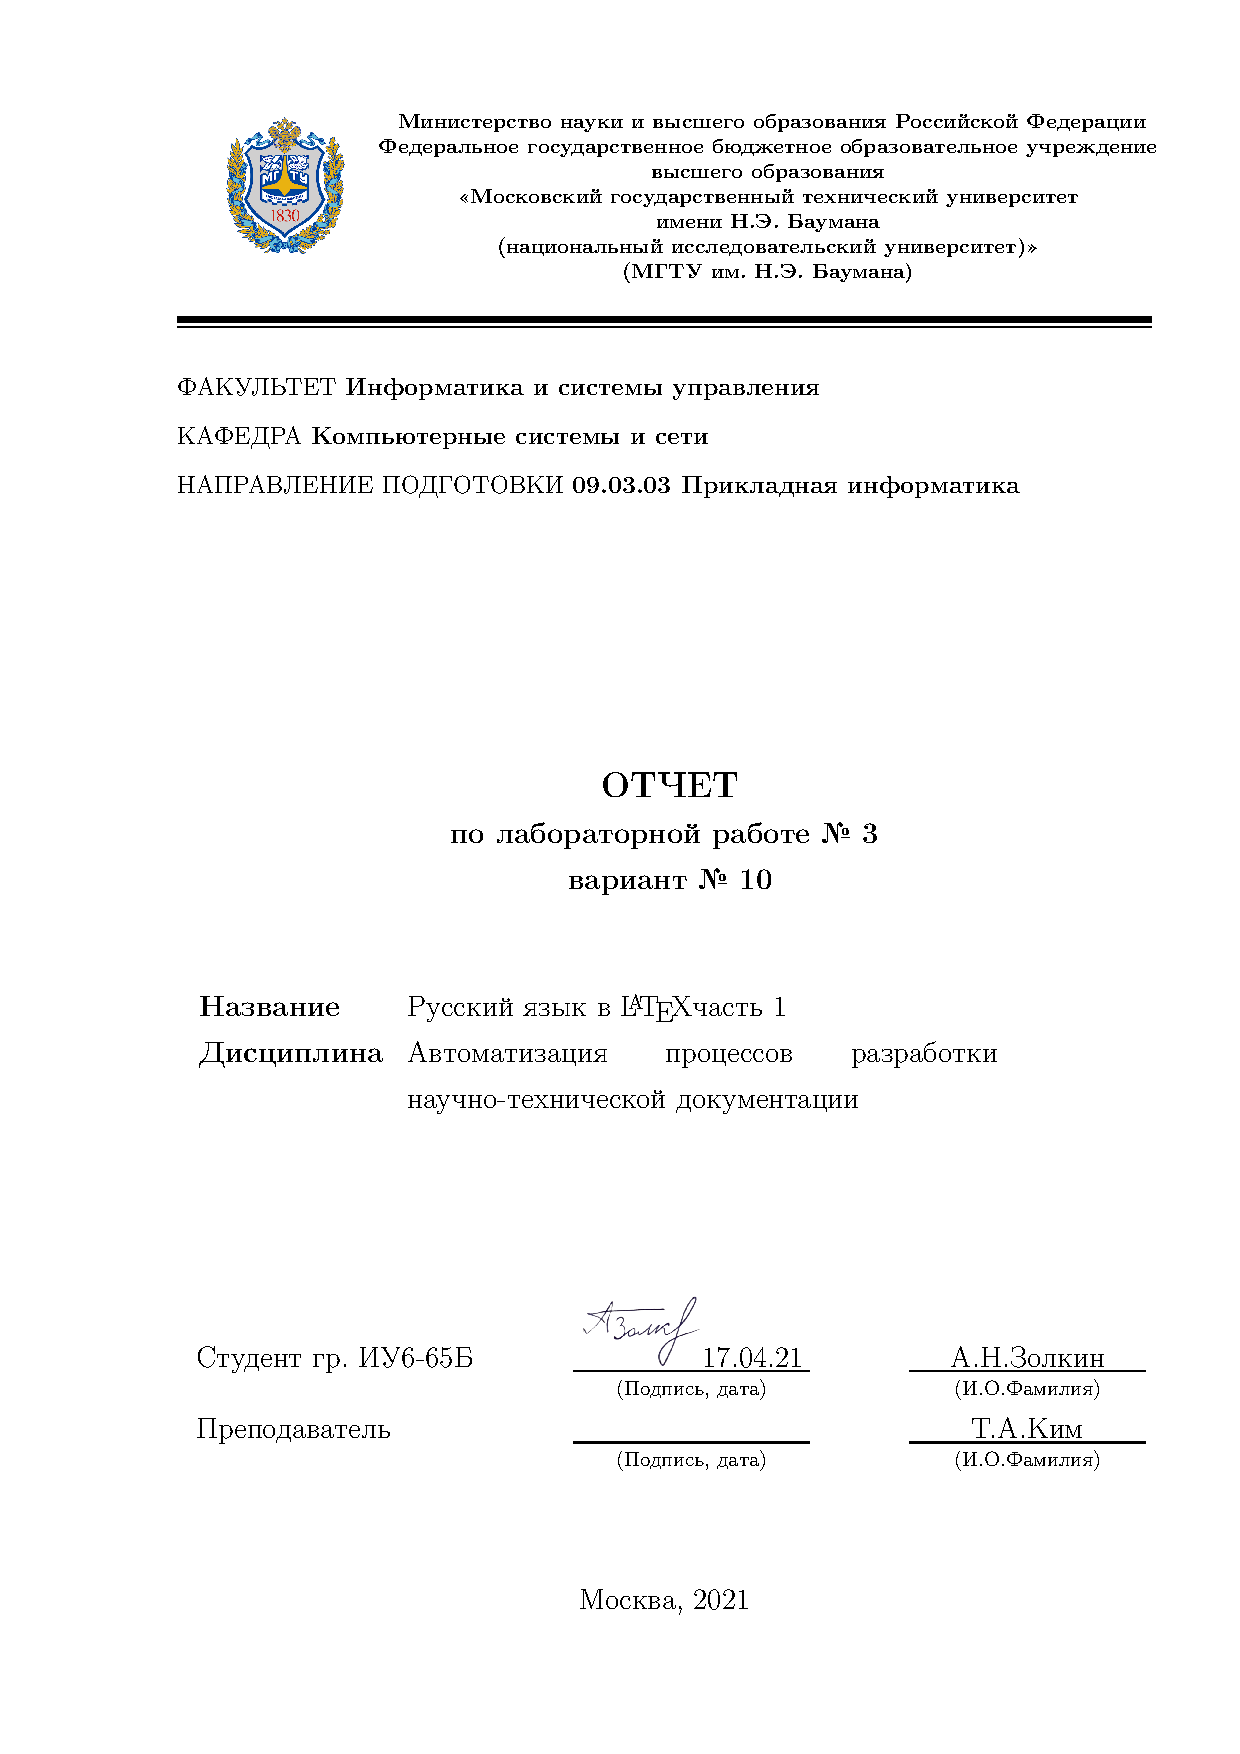
\includepdf[pages=-]{front_page.pdf}
\large{
    \par \textbf{Цель работы}: получить навыки по использованию \LaTeX как инструмента для получения текстов,соответствующих русской типографской традиции.
    \bigskip
    \par Французы атаковали батарею и, увидав Кутузова, выстрелили по нем. С этим залпом полковой командир схватился за ногу; упало несколько солдат, и подпрапорщик, стоявший с знаменем, выпустил его из рук; знамя зашаталось и упало, задержавшись на ружьях соседних солдат.
    \par Солдаты без команды стали стрелять.
    \par "--* Ооох! "--* с выражением отчаяния промычал Кутузов и оглянулся. "--* Болконский, "--* прошептал он дрожащим от сознания своего старческого бессилия голосом. "--* Болконский, "--* прошептал он, указывая на расстроенный батальон и на неприятеля, "--* что ж это?
    \par Но прежде чем он договорил эти слова, князь Андрей, чувствуя слезы стыда и злобы, подступавшие ему к горлу, уже соскакивал с лошади и бежал к знамени.
    \par "--* Ребята, вперед! "--* крикнул он детски-пронзительно.
    \par <<Вот оно!>> думал князь Андрей, схватив древко знамени и с наслаждением слыша свист пуль, очевидно,направленных именно против него. Несколько солдат упало.
    \par "--* Ура! "--* закричал князь Андрей, едва удерживая в руках тяжелое знамя, и побежал вперед с несомненной уверенностью, что весь батальон побежит за ним.
    \par Действительно, он пробежал один только несколько шагов. Тронулся один, другой солдат, и весь батальон с криком <<ура!>> побежал вперед и обогнал его. Унтер-офицер батальона, подбежав, взял колебавшееся от тяжести в руках князя Андрея знамя, но тотчас же был убит. Князь Андрей опять схватил знамя и, волоча его за древко, бежал с батальоном. Впереди себя он видел наших артиллеристов, из которых одни дрались, другие бросали пушки и бежали к нему навстречу; он видел и французских пехотных солдат, которые хватали артиллерийских лошадей и поворачивали пушки. Князь Андрей с батальоном уже был в 20-ти шагах от орудий. Он слышал над собою неперестававший свист пуль, и беспрестанно справа и слева от него охали и падали солдаты. Но он не смотрел на них; он вглядывался только в то, что происходило впереди его "--* на батарее. Он ясно видел уже одну фигуру рыжего артиллериста с сбитым на бок кивером, тянущего с одной стороны банник, тогда как французский солдат тянул банник к себе за другую сторону. Князь Андрей видел уже ясно растерянное и вместе озлобленное выражение лиц этих двух людей, видимо, не понимавших того, что они делали.
    \par <<Что они делают? "--* думал князь Андрей, глядя на них: "--* зачем не бежит рыжий артиллерист, когда у него нет оружия? Зачем не колет его француз? Не успеет добежать, как француз вспомнит о ружье и заколет его>>.
    \par Действительно, другой француз, с ружьем на-перевес подбежал к борющимся, и участь рыжего артиллериста, всё еще не понимавшего того, что ожидает его, и с торжеством выдернувшего банник, должна была решиться. Но князь Андрей не видал, чем это кончилось. Как бы со всего размаха крепкой палкой кто-то из ближайших солдат, как ему показалось, ударил его в голову. Немного это больно было, а главное, неприятно, потому что боль эта развлекала его и мешала ему видеть то, на что он смотрел.
    \par <<Что это? я падаю? у меня ноги подкашиваются>>, подумал он и упал на спину. Он раскрыл глаза, надеясь увидать, чем кончилась борьба французов с артиллеристами, и желая знать, убит или нет рыжий артиллерист, взяты или спасены пушки. Но он ничего не видал. Над ним не было ничего уже, кроме неба "--* высокого неба, не ясного, но всё-таки неизмеримо высокого, с тихо ползущими по нем серыми облаками. << Как тихо, спокойно и торжественно, совсем не так, как я бежал, "--* подумал князь Андрей, "--* не так, как мы бежали, кричали и дрались; совсем не так, как с озлобленными и испуганными лицами тащили друг у друга банник француз и артиллерист, "--* совсем не так ползут облака по этому высокому бесконечному небу. Как же я не видал прежде этого высокого неба? И как я счастлив, я, что узнал его наконец. Да! всё пустое, всё обман, кроме этого бесконечного неба. Ничего, ничего нет, кроме его.
    Но и того даже нет, ничего нет, кроме тишины, успокоения. И слава Богу!. . . >>
}
\bigskip
\texttt{\VerbatimInput[frame=lines, breaklines=true, breakanywhere=true]{lab3}}
\bigskip
\large{
    \par \textbf{Вывод}: В ходе выполнения лабораторной работы были получены навыки по форматированию текста в инструменте \LaTeX. Изучены основы работы с xelatex, использование нескольких tex файлов и подключение уже скомпилированных pdf файлов.
}

\end{document}
